%%%%%%%%%%%%%%%%%%%%%%%%%%%%%%%%%%%%%%%%%%%%%%%%%%%%%%%%%%%%%%%%%%%%%%%%%%%%%%%%
% Presentation contents
%%%%%%%%%%%%%%%%%%%%%%%%%%%%%%%%%%%%%%%%%%%%%%%%%%%%%%%%%%%%%%%%%%%%%%%%%%%%%%%%

\begin{frame}\frametitle{Outline}
\begin{enumerate}
\item Background and motivation.
\item 
\item Section
 \begin{itemize}
  \item Subsection
  \item 
 \end{itemize}
\item Conclusions.
\item References.
\end{enumerate}
\end{frame}

 
\begin{frame}\frametitle{1. Background and Motivation}
 \lipsum[1]
\end{frame} 

\begin{frame} 
 \vspace*{2.0cm}
   \lipsum[1]
\end{frame} 
  
 
 
\begin{frame}\frametitle{2. Section Title}
 \lipsum[1]
\end{frame}
 
\begin{frame}
\vspace*{2.0cm}
\begin{itemize}
 \item The joint posterior distribution over the model and parameter space can be computed based on the Bayes' theorem as \cite{fan_and_sisson_2011},
 \vspace{0.51cm}
 \begin{equation}\label{eq:posterior_models_params}
  f(\mathcal{M}_k, \boldsymbol{\theta}_{k}| \tilde{\mathbf{y}}) = \frac{f(\mathcal{M}_k)f(\boldsymbol{\theta}_{k} | \mathcal{M}_k)L(\tilde{\mathbf{y}} | \mathcal{M}_k, \boldsymbol{\theta}_{k})}{f\left(\tilde{\mathbf{y}}| \mathcal{M}_k\right)}
 \end{equation}
 \vspace{0.5cm}
 where the factor, $f\left(\tilde{\mathbf{y}}| \mathcal{M}_k\right) =\sum_{k\in\mathcal{K}} \int_{\mathbb{R}^{n_k}} f(\mathcal{M}_k) f(\boldsymbol{\vartheta}_{k} | \mathcal{M}_k) L(\tilde{\mathbf{y}} | \mathcal{M}_k, \boldsymbol{\vartheta}_{k}) \dd \boldsymbol{\vartheta}_{k}$, is called the evidence of the model class.
\end{itemize}
\end{frame}
 
 
 
 
\begin{frame} %\frametitle{}
 \vspace*{2.0cm}
 \begin{figure}[!ht]
    \centering
    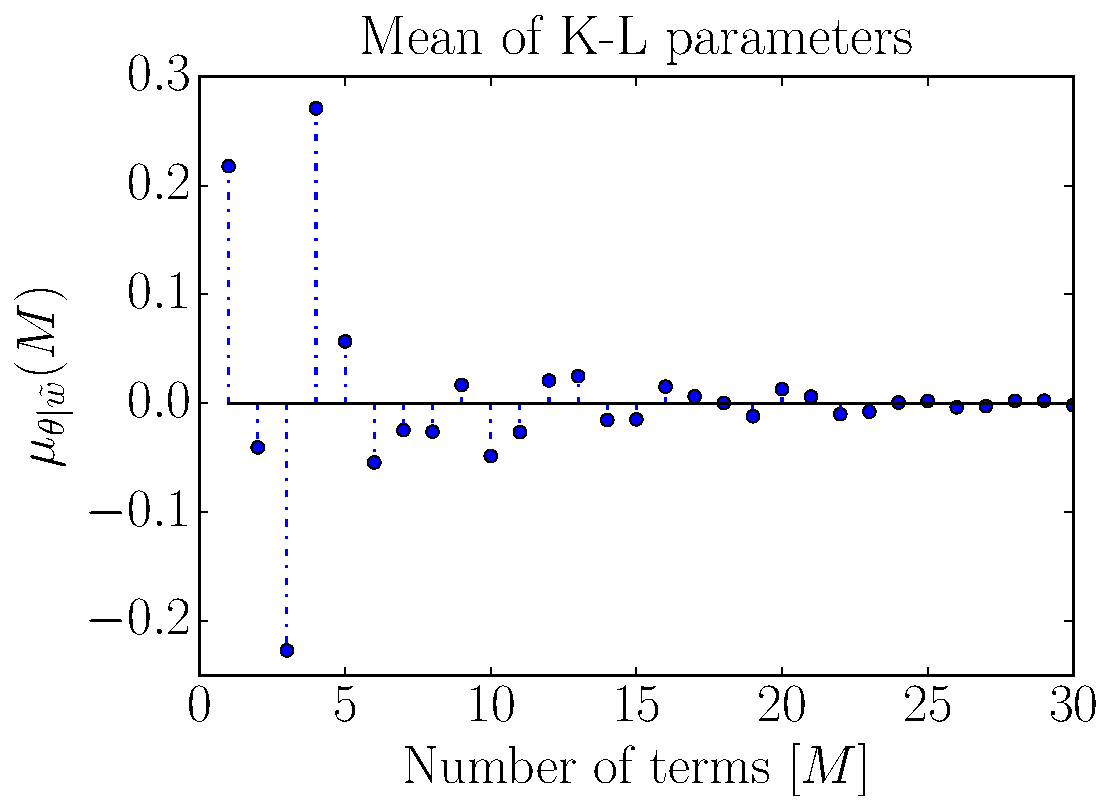
\includegraphics[width=0.6\linewidth]{post_mean_t}
    \caption{Some pic.}
 \end{figure}
\end{frame} 
 
 

\begin{frame}\frametitle{?. Concluding remarks}
\begin{enumerate}
\item[1] Lalala.
\vspace*{1.0cm}

\item[2] Lalalala.
\end{enumerate}
\end{frame} 


\begin{frame}[allowframebreaks]
\vspace*{2.0cm}
  \printbibliography
\end{frame}
